
\chapter{Instrumentazione del sistema}
	
	\section{Installazione e configurazione di Snort}
		
		Il progetto consiste nel valutare il comportamento, dal punto di vista temporale, di Snort come IDS. Andremo ad installare Snort in due macchine che utilizzano come OS Ubuntu 12.04.\\
		Per installare e configurare Snort come IDS è necessario seguire i seguenti passi:
		\begin{itemize}
		  \item \textbf{Scaricare librerie necessarie a Snort}: dobbiamo cioè verificare se nel nostro sistema sono già installate librerie come: libpcap0.8, libpcre3, libdnet-1.12, daq-1.1.1, flex, libpcap-ruby, libtool.
		  \item \textbf{Scaricare la versione aggiornata di Snort} dal sito \textit{http://www.snort.org/\\ snort-downloads} e procediamo con l'installazione vera e propria del software.
		  \item \textbf{Aprire il prompt}, ed eseguire in successione i comandi:
		        \begin{itemize}
		            \item \textit{sudo tar zxvf snort-2.9.4.6.tar.gz}
		            \item \textit{cd snort-2.9.4.6}
		            \item \textit{sudo ./configure --prefix=/usr/local/snort --enable-sourcefire}
		            \item \textit{sudo make}
		            \item \textit{sudo make install}
		            \item \textit{sudo mkdir /var/log/snort}
		            \item \textit{sudo chown snort:snort /var/log/snort}
		        \end{itemize}
		  \item \textbf{Scaricare il file delle regole}: per fare questo eseguiamo i comandi:
		        \begin{itemize}
		            \item \textit{sudo tar zxvf snortrules-snapshot-2946.tar.gz -C /usr/local/snort}
		            \item \textit{sudo mkdir /usr/local/snort/lib/snort\_dynamicrules}
		            \item \textit{sudo cp /usr/local/snort/so\_rules/precompiled/Ubuntu-10-4/i386/2.9.4.6/* /\\ /usr/local/snort/lib/snort\_dynamicrules}
		            \item \textit{sudo touch /usr/local/snort/rules/white\_list.rules}
		            \item \textit{sudo touch /usr/local/snort/rules/black\_list.rules}
		            \item \textit{sudo ldconfig}
		        \end{itemize}
		  \item \textbf{Configurare Snort}: dobbiamo modificare il file di configurazione \textit{snort.conf} eseguendo il comando \textit{sudo gedit /usr/local/snort/etc/snort.conf} e modificare le righe:
		        \begin{itemize}
		            \item \textit{var WHITE\_LIST\_PATH ../rules} e \textit{var BLACK\_LIST\_PATH ../rules} rispettivamente in \textit{var WHITE\_LIST\_PATH /usr/local/snort/rules} e \textit{var BLACK\_LIST\_PATH /usr/local/snort/rules}
		            \item \textit{dynamicpreprocessor directory /usr/local/lib/snort\_dynamicpreprocessor/},\\ \textit{dynamicengine /usr/local/lib/snort\_dynamicengine/libsf\_engine.so} e \\ \textit{dynamicdetection directory /usr/local/lib/snort\_dynamicrules} rispettivamente in \\ \textit{dynamicpreprocessor directory /usr/local/snort/lib/snort\_dynamicpreprocessor/},\\ \textit{dynamicengine /usr/local/snort/lib/snort\_dynamicengine/libsf\_engine.so} e \\ \textit{dynamicdetection directory /usr/local/snort/lib/snort\_dynamicrules}
		        \end{itemize}
		        ed aggiungere nella sezione relativa ai file di output generati, la riga \textit{output alert\_csv: alert.csv default} per far si che il report generato sia già in formato csv (ci tornerà utile in fase di analisi).
		  \item \textbf{Lanciare Snort come IDS}: per lanciare Snort come IDS è necessario eseguire il comando snort come root e specificare:
		      \begin{itemize}
		        \item la rete che s'intende monitorare, per mezzo dell'opzione \textit{-i} seguita dal nome della rete (ad esempio \textit{wifi0} per la rete wifi);
		        \item la richiesta di riportare anche su terminale i pacchetti che trafficano nella rete, usando l'opzione \textit{-dev};
		        \item il percorso in cui Snort andrà a salvare il report degli alert rilevati, usando l'opzione \textit{-l} seguita appunto dal percorso;
		        \item il percorso in cui Snort può trovare il proprio file di configurazione, usando l'opzione \textit{-c} seguita dal percorso.
		      \end{itemize}
		\end{itemize}
		
		Snort è stato così installato e ben configurato su entrambe le macchine che andranno a comporre il sistema su cui faremo l'analisi temporale richiesta.
		
	\section{Tool di fault injection}
	In questa sezione descriviamo le caratteristiche e le opzioni dei vari tool utilizzati per gli esperimenti di fault injection, questi tool dovranno essere installati sulla macchina che svolgerà il ruolo di attaccante (nodo B).
	
	\subsection{NMap}
	Nmap ("Network Mapper") è uno strumento open source per la network exploration e l'auditing. \'E stato progettato per scansionare rapidamente reti di grandi dimensioni, ma è indicato anche per l'utilizzo verso singoli host. Nmap usa pacchetti IP raw (grezzi, non formattati) in varie modalità per determinare quali host sono disponibili su una rete, che servizi (nome dell'applicazione e versione) vengono offerti da questi host, che sistema operativo (e che versione del sistema operativo) è in esecuzione, che tipo di firewall e packet filters sono usati, e molte altre caratteristiche.
	L'output di Nmap è uno scan di un elenco di obiettivi, con informazioni supplementari per ognuno a seconda delle opzioni usate. Tra queste informazioni è vitale la ``tabella delle porte interessanti''. Questa tabella elenca il numero della porta e il protocollo, il nome del servizio, e il suo stato attuale.  La tabella delle porte può anche includere dettagli quali le versioni dei software disponibili se è stata usata l'opzione appropriata.\\
	Installare \textit{nmap} è semplicissimo: sarà sufficiente digitare il comando \textit{sudo apt-get install nmap} sul terminale.\\
	Negli esperimenti abbiamo scelto di valutare il comportamento di Snort soggetto ad attacchi generati con \textit{nmap} e le seguenti opzioni:
	\begin{itemize}
	    \item \textit{ --osscan\_guess (Guess OS detection results)}, con questa opzione attiva se nmap non è in grado di rilevare una corrispondenza esatta dell'OS, propone come possibilità gli OS più vincini alla rilevazione.\\ La corrispondenza però deve essere molto simile perchè Nmap lo faccia per default. Entrambe queste opzioni (equivalenti) fanno si che Nmap proceda con il riconoscimento dell'OS in modo più aggressivo.
	    \item \textit{--version\_light (Attiva la modalità Light)}, questa modalità rende il Version Scanning drasticamente più veloce, riducendone però la capacità di identificare accuratamente i servizi.
	    \item \textit{--version\_all (Prova ogni singolo pacchetto-sonda)},questa opzione assicura che ogni singolo pacchetto-sonda venga utilizzato su ogni singola porta.
	    \item \textit{-T (Imposta un template di temporizzazione)}, tramite questa opzione nmap offre un approccio per il testing più semplice, lo fa mediante sei "timing templates", ovvero opzioni pre-impostate per regolare l'aggressività della scansione. Esse si specificano mediante l'opzione -T seguita dal numero del template
	           corrispondente o dal suo nome. Essi sono: paranoico (0), furtivo (1), educato (2), normale (3), aggressivo (4) e folle (5). I primi due vengono usati per evitare i sistemi anti-intrusione (IDS). La modalità "gentile" rallenta la scansione in modo da usare meno banda e risorse sulla macchina bersaglio. La modalità  "normale" è di default (e pertanto l'opzione -T3 non modifica nulla). La modalità "aggressiva" incrementa la velocità assumendo che si è su una rete veloce ed affidabile. Infine la modalità "folle" dà per scontato che si è su una rete estremamente veloce ed affidabile o che si vuole sacrificare l'accuratezza in nome della velocità.
	
	    \item \textit{-A (Opzioni di scan aggressive)}, questa opzione abilita opzioni addizionali avanzate e aggressive.
	
	    \item \textit{-sn}, esegue una scansione ping ed esclude la scansione sulle porte.\\Questo comando è stato testato, tra i vari esperimenti condotti in questo lavoro, ma non è stato rilevato in alcun modo da Snort, né sotto forma di alert né come pacchetti ricevuti. Quindi questo particolare attacco è stato escluso nella fase di analisi.
	
	
	\end{itemize}
	
	\subsection{Ping}
	Ping verifica le connessioni a computer remoti. Invia pacchetti di echo ICMP Internet Control Message Protocol a un computer e attende i pacchetti di risposta. Ping attende di default fino a 1 secondo per ogni pacchetto inviato e viene stampato il numero di pacchetti trasmessi e ricevuti sulla console. L'attesa per ogni pacchetto inviato essere specificata utilizzando l'opzione \textit{-i}
	Il comando \textit{ping} è già disponibile all'interno della distribuzione Ubuntu utilizzata.\\
	Per i nostri esperimenti andremo ad utilizzare l'opzione \textit{-i} del comando, tale opzione permette di esplicitare l'intervallo di tempo da attendere tra l'invio di ogni pacchetto. Il valore di default è un secondo, o non attendere in modalità \textit{flood}. Solo un super-utente può impostare l'intervallo  a valori inferiori di 0,2 secondi.\\
	Per verificare la variazione di funzionamento di Snort a seguito di pacchetti inviati più velocemente abbiamo creato una nuova regola:\\
	\\
	\textit{alert icmp any any -> 192.168.137.180 any (msg:``TOO MUCH PING''; threshold: type both, track by\_src, count 10, seconds 3; classtype:attempted-dos; sid:51000; rev:2;)}\\
	\\	
	Tale regola ci permette di discriminare il comportamento tenuto da Snort al variare del valore per l'opzione \textit{-i}.
	
	
	\subsection{Metasploit}
	Metasploit Project è un progetto open source (rilasciato con licenza BSD) dedicato alla sicurezza informatica il quale fornisce informazioni sulle vulnerabilità della rete e ne semplifica le operazioni di penetration testing e ne aiuta nello sviluppo di sistemi di rilevamento di intrusioni.
	Assieme al progetto Metasploit troviamo anche Metasploit Framework uno strumento dedicato principalmente allo sviluppo e l'esecuzione di exploit ai danni di una macchina remota.
	Sono messe a disposizioni varie interfaccie ma nel seguito andremo ad utilizzare l'interfaccia web msfweb, utile per usare il framework con tutta la comodità di un'interfaccia web.
	Metasploit Project viene rilasciato con un semplice installar il quale ci permetterà d'installare l'applicazione in qualsiasi distribuzione Linux.
	Per installare Metasploit Project su OS Ubuntu basta digitare:
	\begin{itemize}
	\item \textit{wget http://downloads.metasploit.com/data/releases/metasploit-latest-linux-installer.run}
	\item \textit{chmod +x metasploit-latest-linux-installer.run}
	\item \textit{sudo ./metasploit-latest-linux-installer.run}
	\end{itemize}
	a questo punto si aprirà un wizard con il quale procederemo all'installazione di Metasploit e in cui ci verrà chiesto d'inserire la porta SSL dedicata al servizio e successivamente la creazione dei certificati SSL.\\
	Al termine del Wizard d'installazione potremo accedere alla Web Ui di Metasploit la qual ci confermerà la corretta installazione. Potremo a questo punto lanciare l'interfaccia web di Metasploità dove sarà richiesto di creare ed attivare un account.\\
	Per i nostri esperimenti si è scelto di utilizzare \textit{metasploit} come \textit{port scan}, sarà necessario digatere l'indirizzo ip su cui eseguire la scansione e successivamente specificare le varie opzioni avanzate per la scansione. Le scansioni che effettueremo sono essenzialmente due, quella di default senza specificare alcuna opzione avanzata e una seconda in cui abiliteremo la \textit{Scan SNMP community strings Information}: quest'opzione lancia un task in background per analizzare i device SNMP che corrispondono ad una serie di stringhe (essendo un lavoro generalmente lungo, viene eseguito in parallelo con le altre scansioni base).
	
	\subsection{Traceroute}
	\textit{Traceroute} cerca di tracciare il percorso seguito dai pacchetti IP per un qualche host internet. Cerca i passaggi intermedi, lanciando pacchetti sonda con un piccolo TTL, e quindi resta in ascolto di un \textit{ICMP reply} da un router intermedio. \textit{Traceroute} inizia la rilevazione con un TTL di uno, e lo incrementa fino a quando viene ricevuto un \textit{ICMP port unreachable reply}. Questo significa che la sonda o ha raggiunto l'host, o ha raggiunto il TTL massimo.\\
	Per rendere disponibile questo tool, se non già presente tra le librerie dell'OS, è necessario eseguire il comando \textit{apt-get install traceroute} tramite il quale sarà installato e quindi reso disponibile.\\
	Negli esperimenti andremo ad attivare alternativamente le seguenti opzioni:
	\begin{itemize}
	    \item \textit{-I (icmp)}, abilita il comportamento ad ora usuale per traceroute, utilizzando pacchetti ICMP ECHO per le sonde.
	    \item \textit{-T (tcp)}, abilita un nuovo comportamento per traceroute destinato ad aggirare i firewall.\\ Utilizza una porta di destinazione costante (di default è 80, http).\\
	        Questo metodo utilizza la ben nota "\textit{half-open technique}", che impedisce alle applicazioni sull'host di destinazione di far vedere le nostre sonde a tutti.\\
	        Includendo l'opzione -T all'attacco con traceroute, Snort rileva (sul nodo A) una serie di pacchetti in arrivo ma non genera alcun tipo ti alert (o perché l'attacco viene considerato innocuo, o perché Snort non ha regole sufficienti a rilevarlo). Nella fase di analisi, quindi, sono state escluse le misurazioni sui tempi di detection che riguardano quest'esperimento.
	
	    \item \textit{-N (squeries)}, Specifica il numero di pacchetti sonda inviati simultaneamente.\\
	    L'invio di più sonde contemporaneamente può accelerare notevolmente traceroute (il valore predefinito è 16). Si noti che alcuni router e gli host possono utilizzare \textit{ICMP  rate  throttling}e in una tale situazione specificando un numero troppo grande si può avere la perdita di alcune risposte.
	\end{itemize}
	
	\section{Tool di data integration e analisi}
	In questa ultima sezione andiamo a descrivere il tool che utilizzeremo per integrare e manipolare i dati raccolti al fine di generare successivamente un sistema OLAP su cui effettuare tutte le analisi.\\
	Il framework utilizzato è \textit{Pentaho}, precisamente il tool \textit{Kettle} per la \textit{Data Integration} ed il motore MOLAP \textit{Mondrian} per analisi di tipo OLAP.\\
	Il framework messo a disposizione da Pentaho permette di sviluppare soluzioni complete per la \textit{Business Intelligence} ma noi ci limiteremo ad utilizzare i tool sopra citati, che sono ampiamente sufficienti per soddisfare le nostre richieste.\\
	Utilizzando il tool \textit{Kettle}, è possibile integrare e manipolare i file \textit{.csv} generati in fase sperimentale, così da renderli in una forma più consona alla memorizzazione all'interno di un database, ad esempio sarà possibile dividere il campo relativo al timestamp nelle sue sottocomponenti, così da rendere più semplice la correzione del tempo indicata dall'offset di sfasamento degli orologi rilevato tramite il comando \textit{ntpdate} oppure ancora permette di aggiungere nuovi campi come ad esempio ``EXP\_ID'' che andrà a identificare univocamente i pacchetti relativi ad un determinato esperimento.
	Vediamo qui la trasformazione (per comodità divisa in quattro immagini) che permetterà di integrare tra loro i dati relativi ai vari esperimenti eseguiti:
	
	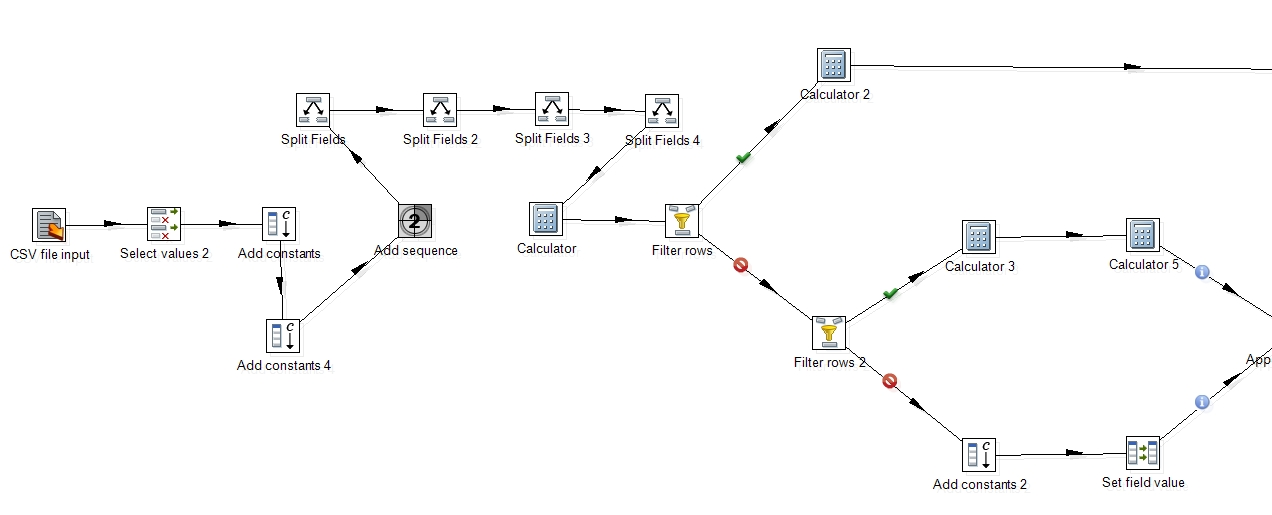
\includegraphics[scale=0.4]{figure/kettle1.jpg}\\
	
	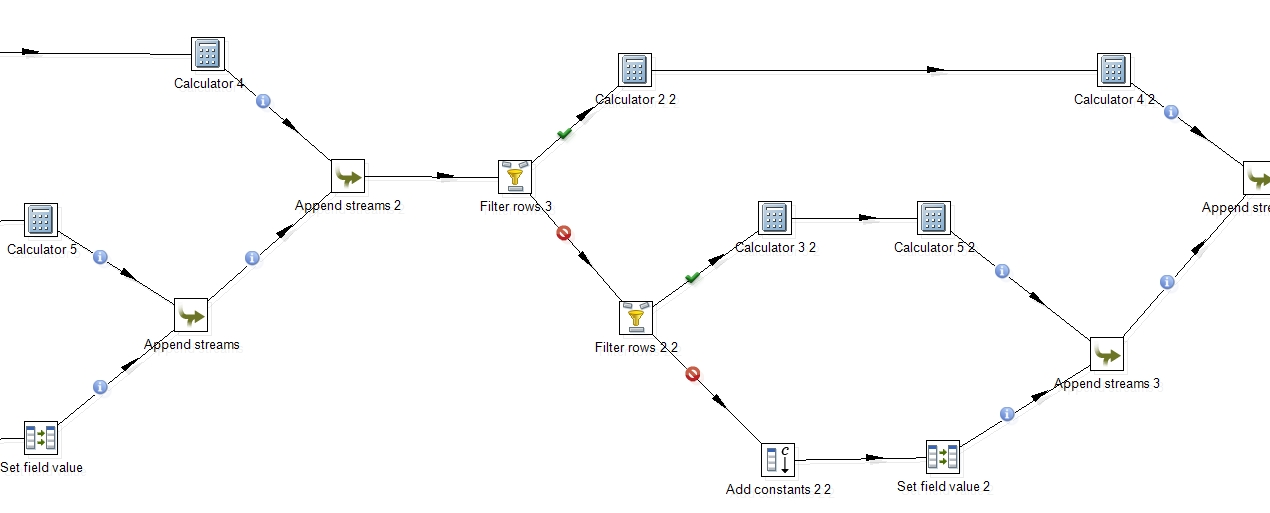
\includegraphics[scale=0.4]{figure/kettle2.jpg}\\
	
	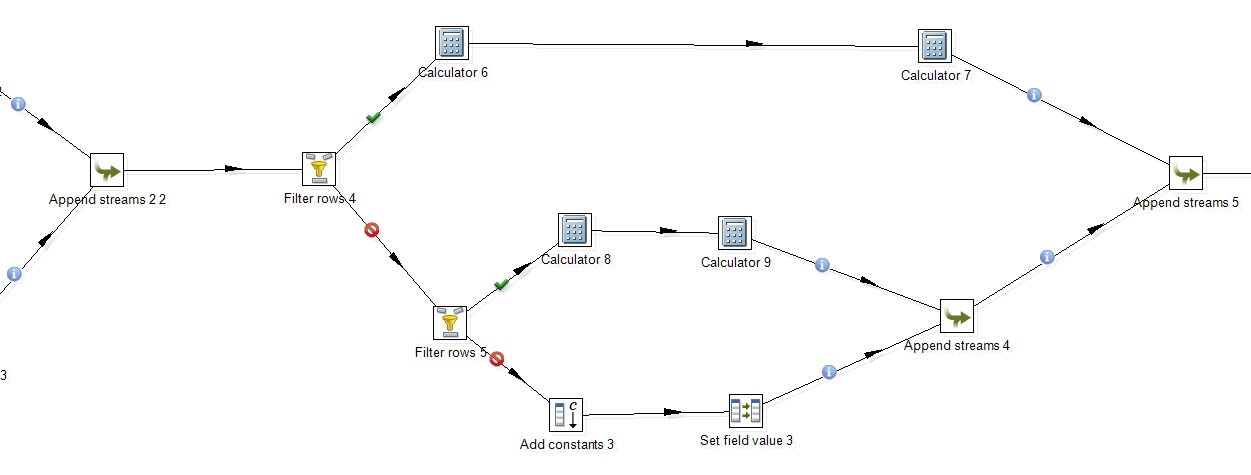
\includegraphics[scale=0.4]{figure/kettle3.jpg}\\
	
	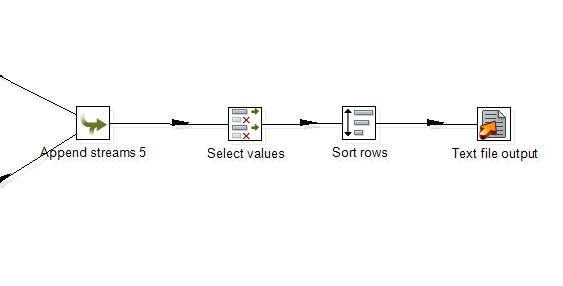
\includegraphics[scale=0.4]{figure/kettle4.jpg}
	
	Il file generato da Kettle (file di log \textit{logCompleto.csv}), ancora in formato \textit{.csv}, consisterà nell'elenco di tutti i pacchetti loggati a cui sono associate tutte le informazioni registrate durante gli esperimenti. Ovviamente tale file è spesso e volentieri ridondante, proprio come chiede la logica OLAP.\\
	A questo punto utilizzando il tool \textit{Mondrian} è possibile definire uno \textit{star-schema}, che avrà la struttura indicata in Figura \ref{fig:star}.
	
	\begin{figure}[h!]
		\centering
		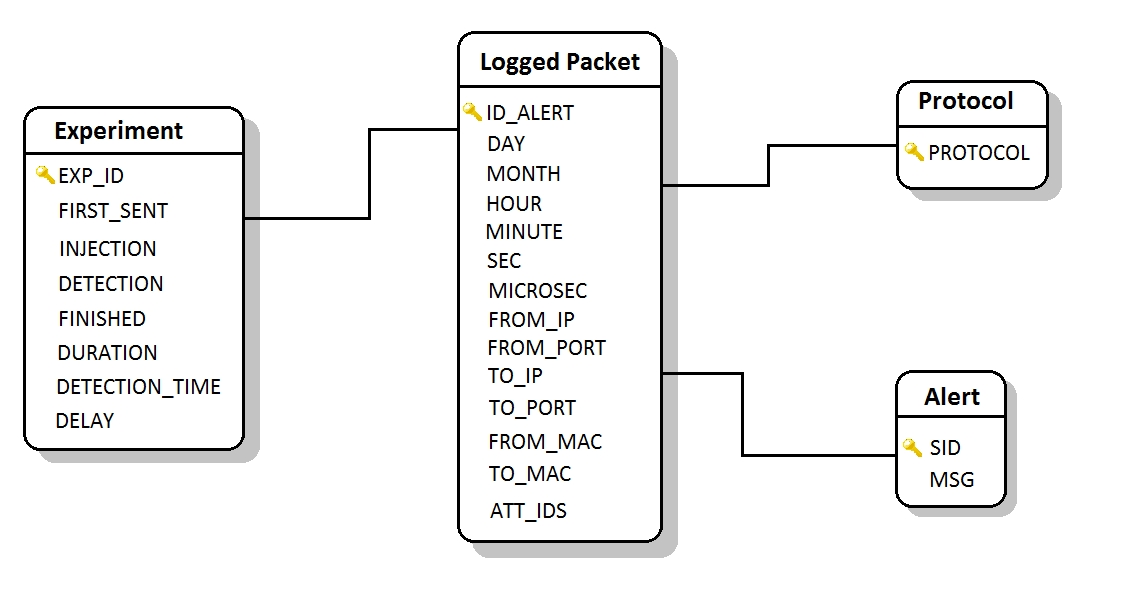
\includegraphics[scale=0.45]{figure/star-schema.jpg}
		\caption{\textit{Schema a stella} costruito sul file di log finale.}
		\label{fig:star}
	\end{figure}
	
	Questa struttura ci permetterà di modellare il fatto "\textit{Logged Packet}". L'analisi, infatti, è volta ad analizzare come Snort reagisce e varia le proprie prestazioni al variare sia di tool di fault injection che, pur rimanendo all'interno dello stesso tool, delle opzioni attive.\\
	Prima di caricare nel database tutte le informazioni contenute nel file \textit{.csv}, per velocizzare il processo di analisi utilizzeremo un semplice programma \textit{Java} (Codice \ref{lst:java}, Appendice A), il quale, analizzando il file generato da \textit{Kettle}, permetterà di calcolare le seguenti tempistiche necessarie per l'analisi:
	\begin{itemize}
	    \item L'istante di tempo in cui l'attacco è generato dal nodo B.
	    \item L'istante di tempo in cui l'attacco è iniettato sul nodo A.
	    \item L'istante di tempo in cui l'attacco è individuato da parte di Snort.
	    \item Il ritardo di trasmissione introdotto dalla rete.
	    \item Il tempo di \textit{detection}, cioè il tempo impiegato da Snort per rilevare l'attacco.
	    \item La durata dell'attacco.
	\end{itemize}
	
	Questi tempi, per una più semplice manipolazione, saranno ``assoluti'' cioè si riferiranno ad uno stesso giorno di uno stesso mese e l'orario sarà espresso in microsecondi. Ogni esperimento avrà ovviamente proprie tempistiche.\\
	Arrivati a questo punto tutti i dati raccolti e le quantità necessarie per l'analisi saranno nella forma più adatta per la memorizzazione in un database (file di log \textit{logFinale.csv}). Procederemo con l'analisi per mezzo di funzioni OLAP rese disponibili anch'esse nel framework \textit{Pentaho}, precisamente usando \textit{Mondrian}. Sarà così semplice fornire grafici o report di ogni tipo incrociando a piacimento i dati raccolti per i vari esperimenti.
	Riporteremo le analisi effettuate nei seguenti capitoli. Occorre però osservare che il numero di comparazioni effettuabili sono molteplici e tutte facilmente ottenibili utilizzando \textit{Pentaho}, sfruttando la ridondanza creata per mezzo di \textit{kettle} nel file \textit{.csv} che svolge la funzione di repositary dei dati sperimentali.
